\section{Introduction}
SAML simplifies federated authentication and authorization processes for users,
Identity providers, and service providers. SAML provides a solution to allow
your identity provider and service providers to exist separately from each
other, which centralizes user management and provides access to SaaS
solutions.

SAML implements a secure method of passing user authentications and
authorizations between the identity provider and service providers. When a user
logs into a SAML enabled application, the service provider requests
authorization from the appropriate identity provider. The identity provider
authenticates the user’s credentials and then returns the authorization for the
user to the service provider, and the user is now able to use the application.

SAML authentication is the process of verifying the user’s identity and
credentials (password, two-factor authentication, etc.). SAML authorization
tells the service provider what access to grant the authenticated user.

\begin{figure}
  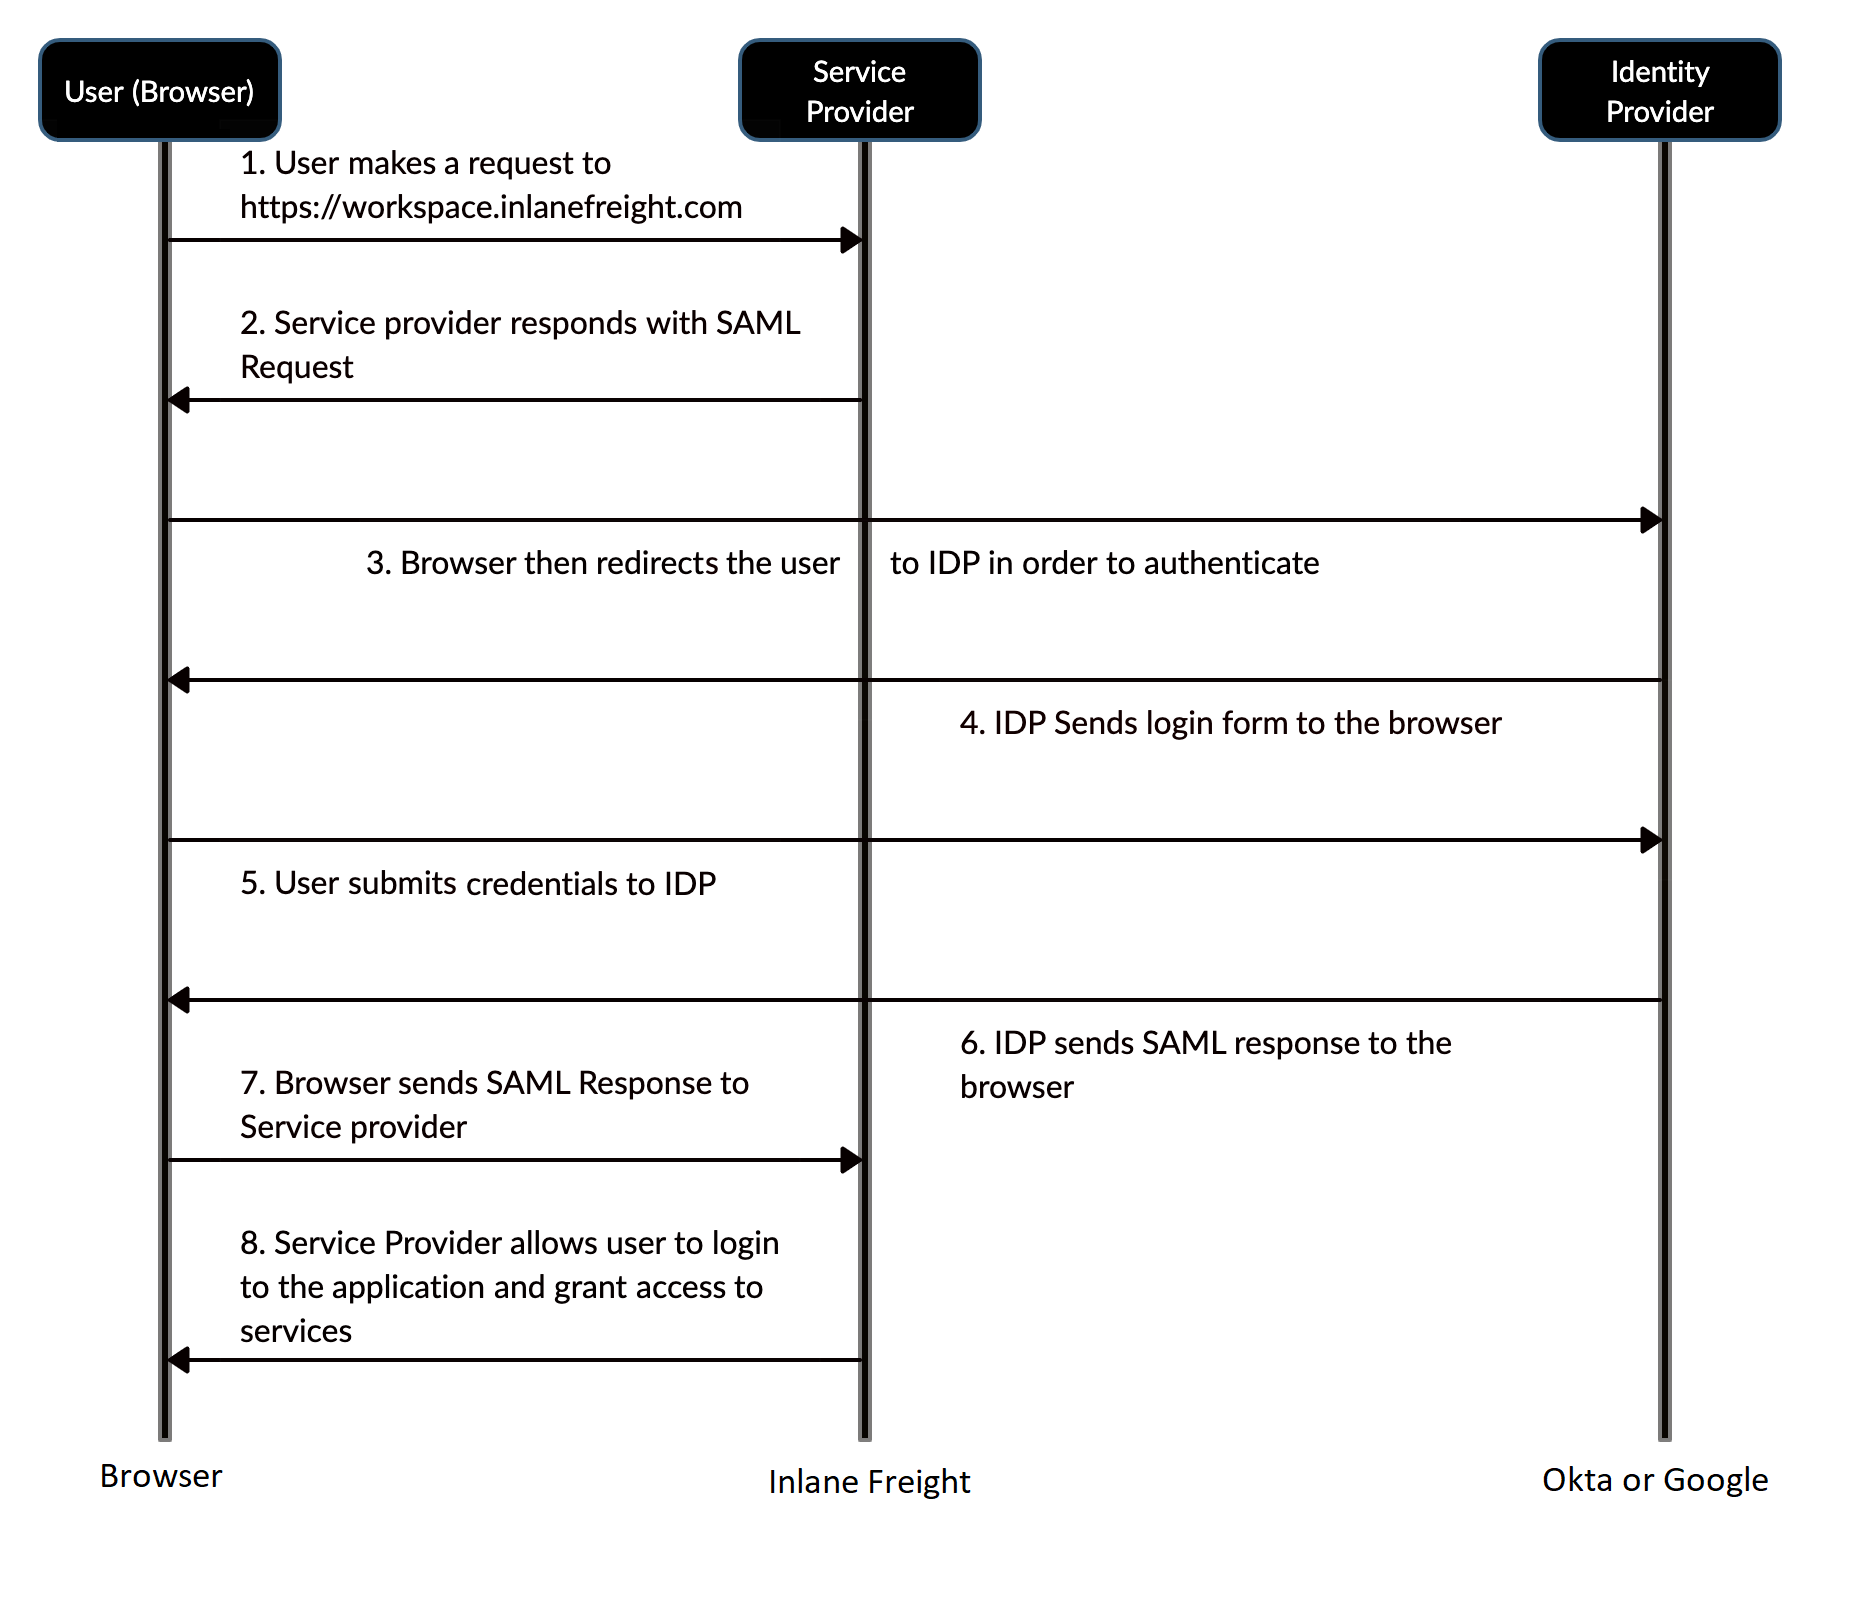
\includegraphics[width=\linewidth]{web_server_side/saml/images/saml-flow.png}
  \caption{SAML v2 flow}
  \label{fig:saml-flow}
\end{figure}

\subsection{SAML request}

Consider making a request to a ressource located at SP
\verb+https://shibdemo-sp1.test.edu/secure/+

\begin{verbatim}
GET /secure/ HTTP/1.1
Host: shibdemo-sp1.test.edu
User-Agent: Mozilla/5.0 (X11; Ubuntu; Linux x86_64; rv:65.0) Gecko/20100101 Firefox/65.0
Accept: text/html,application/xhtml+xml,application/xml;q=0.9,image/webp,*/*;q=0.8
Accept-Language: en-US,en;q=0.5
Accept-Encoding: gzip, deflate
Referer: https://shibdemo-sp1.test.edu/
Connection: close
Upgrade-Insecure-Requests: 1
\end{verbatim}

The SP generates a SAML Request because we’re not authenticated. We can see the
raw SAML Request below:
\begin{verbatim}
<?xml version="1.0"?>
<samlp:AuthnRequest
    xmlns:samlp="urn:oasis:names:tc:SAML:2.0:protocol"
    AssertionConsumerServiceURL="https://shibdemo-sp1.test.edu/Shibboleth.sso/SAML2/POST"
    Destination="https://shibdemo-idp.test.edu/idp/profile/SAML2/Redirect/SSO"
    ID="_cdae718238ba9c207a35cc7c70b046a0"
    IssueInstant="2019-03-12T20:54:58Z"
    ProtocolBinding="urn:oasis:names:tc:SAML:2.0:bindings:HTTP-POST"
    Version="2.0">
    <saml:Issuer xmlns:saml="urn:oasis:names:tc:SAML:2.0:assertion">
        https://shibdemo-sp1.test.edu/shibboleth
    </saml:Issuer>
    <samlp:NameIDPolicy AllowCreate="1"/>
</samlp:AuthnRequest>
\end{verbatim}

key attributes:
\begin{itemize}
    \item \verb+AssertionConsumerServiceURL+ Identifies where the IdP should
        send the SAML Response to after authentication.
    \item \verb+Destination+: Indicates the address to which the request should
        be sent (IdP).
    \item \verb+ProtocolBinding+: Typically accompanies the
        \verb+AssertionConsumerServiceURL+ attribute and defines the mechanism
        by which SAML protocol messages will be transmitted.
    \item \verb+saml:Issuer+: Identifies the entity that generated the request
        message.
\end{itemize}

With the SAML Request created, the SP now replies to our GET request for
\verb+/secure/+ with a 302 redirect. The 302 directs our browser to head over
to the IdP. The SAML Request is encoded into the HTTP response’s Location
header as part of the 302.

\begin{verbatim}
HTTP/1.1 302 Found
Date: Tue, 12 Mar 2019 20:54:58 GMT
Server: Apache/2.2.3 (CentOS)
Expires: Wed, 01 Jan 1997 12:00:00 GMT
Cache-Control: private,no-store,no-cache,max-age=0
Location: https://shibdemo-idp.test.edu/idp/profile/SAML2/Redirect/SSO?SAMLRequest=fZJdT4MwFIb%2FCuk9FNgmWzNIcLtwyXRkoBfemFKO0gRa7Cl%2B%2FHvZmDoTs8u2b5%2B350mXyNumY2lva7WH1x7QOh9to5AdD2LSG8U0R4lM8RaQWcHy9HbLQs9nndFWC90QJ0UEY6VWK62wb8HkYN6kgPv9Nia1tR0ySrGWZQWtdrELPDs0eVD1NB92S92ArT1ETQ%2FwkGa7vCDOeshIxQ%2Fcfyiy6n4pw4IOz3mWDZwQe6ikAWFpnu%2BIs1nH5ElUHKJgHk7mJV%2BI0I%2F4ZCZEJCK%2F9KdX3B9iiD1sFFqubExCP1i4%2FsQNwiL02WzKZvNH4mSnqa%2BlqqR6uayoHEPIbooic8exHsDgcaQhQJLlQTQ7Fpsz9Zex%2FNs3SS7bxR%2B7S3pWNLZ27G4gb9aZbqT4dNKm0e8rA9xCTAJCk%2FHK39%2BRfAE%3D&RelayState=ss%3Amem%3A39430bdac29d44586c326f12b4cb3345ffa47137a374e37cba0877e0fc79ea91
Content-Length: 897
Connection: close
Content-Type: text/html; charset=iso-8859-1

<!DOCTYPE HTML PUBLIC "-//IETF//DTD HTML 2.0//EN">
<html><head>
<title>302 Found</title>
</head><body>
<h1>Found</h1>
<p>The document has moved <a href="https://shibdemo-idp.test.edu/idp/profile/SAML2/Redirect/SSO?SAMLRequest=fZJdT4MwFIb%2FCuk9FNgmWzNIcLtwyXRkoBfemFKO0gRa7Cl%2B%2FHvZmDoTs8u2b5%2B350mXyNumY2lva7WH1x7QOh9to5AdD2LSG8U0R4lM8RaQWcHy9HbLQs9nndFWC90QJ0UEY6VWK62wb8HkYN6kgPv9Nia1tR0ySrGWZQWtdrELPDs0eVD1NB92S92ArT1ETQ%2FwkGa7vCDOeshIxQ%2Fcfyiy6n4pw4IOz3mWDZwQe6ikAWFpnu%2BIs1nH5ElUHKJgHk7mJV%2BI0I%2F4ZCZEJCK%2F9KdX3B9iiD1sFFqubExCP1i4%2FsQNwiL02WzKZvNH4mSnqa%2BlqqR6uayoHEPIbooic8exHsDgcaQhQJLlQTQ7Fpsz9Zex%2FNs3SS7bxR%2B7S3pWNLZ27G4gb9aZbqT4dNKm0e8rA9xCTAJCk%2FHK39%2BRfAE%3D&amp;RelayState=ss%3Amem%3A39430bdac29d44586c326f12b4cb3345ffa47137a374e37cba0877e0fc79ea91">here</a>.</p>
<hr>
<address>Apache/2.2.3 (CentOS) Server at shibdemo-sp1.test.edu Port 443</address>
</body></html>
\end{verbatim}

The \verb+RelayState+ parameter sent along with the SAML Request is state
information sent by the SP to the IdP so that the SP knows who initially asked
for the resource when the SAML Response comes back. The SAML Response must
contain the same \verb+RelayState+ value.

The \verb+SAMLRequest+ parameter is a compressed and encoded version of the
same raw xml snippet we looked at earlier. SAML uses the
\href{https://en.wikipedia.org/wiki/DEFLATE}{Deflate compression} algorithm
then base64 encodes the result.

\subsection{SAML response}

\begin{verbatim}
<?xml version="1.0" encoding="UTF-8"?>
<samlp:Response Destination="https://shibdemo-sp1.test.edu/Shibboleth.sso/SAML2/POST" ID="_2af3ff4a06aa82058f0eaa8ae7866541" InResponseTo="_cdae718238ba9c207a35cc7c70b046a0" IssueInstant="2019-03-12T20:54:54.061Z" Version="2.0" xmlns:samlp="urn:oasis:names:tc:SAML:2.0:protocol">
    <saml:Issuer Format="urn:oasis:names:tc:SAML:2.0:nameid-format:entity" xmlns:saml="urn:oasis:names:tc:SAML:2.0:assertion">https://shibdemo-idp.test.edu/idp/shibboleth</saml:Issuer>
    <ds:Signature xmlns:ds="http://www.w3.org/2000/09/xmldsig#">
    <ds:SignedInfo>
      <ds:CanonicalizationMethod Algorithm="http://www.w3.org/2001/10/xml-exc-c14n#"/>
      <ds:SignatureMethod Algorithm="http://www.w3.org/2000/09/xmldsig#rsa-sha1"/>
      <ds:Reference URI="#_2af3ff4a06aa82058f0eaa8ae7866541">
        <ds:Transforms>
          <ds:Transform Algorithm="http://www.w3.org/2000/09/xmldsig#enveloped-signature"/>          <ds:Transform Algorithm="http://www.w3.org/2001/10/xml-exc-c14n#"/>
        </ds:Transforms>
        <ds:DigestMethod Algorithm="http://www.w3.org/2000/09/xmldsig#sha1"/>
        <ds:DigestValue>Se+WwXd5r44J56LauTz/wnP3jWg=</ds:DigestValue>
      </ds:Reference>
    </ds:SignedInfo>
    <ds:SignatureValue>f8X28hHMpnTi/Hqi6phuxqbYKsf99Qi8QqVI3x3zRj6njs+J9ey7qxw4GTMV657IfmmMotE0IAIrmPh3lebX65bCUCpiDtFaP04KjWNGGWa7z6rjwhRIY6chYGYzdmrXWmvY2EXW3nkynAJ2vXo5mncOz2P17/bQgqDU6BTzfRzYU6q6TcGLjRd7pGMGbBm6wH5c8aHM4FaQZNv7qHkIVvTlCRcpg/b8qS2fWW8kwgklLXd1xTCXh9XedxrFWq75nSFZ6FiakfUMybC5YIqZ7nr4GfVKqdmh3wvCF/P9jrUkBNDsw3Id63UAwbnMVvBAYt2tgfiD5hpJ3ZLkzjds+g==</ds:SignatureValue>
    <ds:KeyInfo>
      <ds:X509Data>
        <ds:X509Certificate>MIIDXTCCAkWgAwIBAgIJAO7P8i9TJMuvMA0GCSqGSIb3DQEBCwUAMEUxCzAJBgNVBAYTAkFVMRMwEQYDVQQIDApTb21lLVN0YXRlMSEwHwYDVQQKDBhJbnRlcm5ldCBXaWRnaXRzIFB0eSBMdGQwHhcNMTgwNDA1MDI1NTUyWhcNMjgwNDA0MDI1NTUyWjBFMQswCQYDVQQGEwJBVTETMBEGA1UECAwKU29tZS1TdGF0ZTEhMB8GA1UECgwYSW50ZXJuZXQgV2lkZ2l0cyBQdHkgTHRkMIIBIjANBgkqhkiG9w0BAQEFAAOCAQ8AMIIBCgKCAQEAwfSJJxxWvJ2Xok+Qx1OwQa+LA6mTSomOrgcJkRhfjeA9LMBmQlZKMdHiwKCaJBm7l1G13CNN2XhBZBqLFEX/4pPO5WBakAEa8h1i1ODmge1NKntcr3jPG8pGrzQVFbTpyoPaeJM5nSJUJhdI+QlXEYRZ2WUpKrrPXaG4O/bKFQ4FP7tRiYMi7SZde0QOUSTUlO14JA5L3jNUk0eha2hVULyCEa9WjbfOfw+0TvE32MrAhsu4QJQgr18q1x4+GNuOI0LkX1/WehXDstyjX68CxHRSNfsarX7HeOvqn8HbGkIAKMG1ldmSkyvJ0DrvEU+0wTxaTXxFR+zwFOBnSKIVBwIDAQABo1AwTjAdBgNVHQ4EFgQUn3h8qx+ssGm8balncHSF9hi01NQwHwYDVR0jBBgwFoAUn3h8qx+ssGm8balncHSF9hi01NQwDAYDVR0TBAUwAwEB/zANBgkqhkiG9w0BAQsFAAOCAQEAuVmxbUhFA8cdnxgwHWYXniebXpPNMfoMBPpMao20uv9dkKHH2AzuT7TWAICiSj29ZuHEVJaK1mfwErr+R8etKnGT0tA53/509+gWG0eCQSh+AF/VPWQ4JRoPMszKdLzl4surnNOA5JegKVvTcT91+G+OWv0hB4iMD/quegLSBfrlbtyTT58Moj33wDDhaMH1Dlm23zfgB/0w3ztZnnmdxXJxGZuLiybJXTMbkjhUk41udHTQcsxKdaRoaQobDNdbqyl245RP15QXKphaz8DadCyH4v8o5NIU5lZyEG7KCpWnqWe6au6OrbGqBkqDIrEue3Wnu+TFaJRXBd12D9Xb8g==</ds:X509Certificate>
      </ds:X509Data>
    </ds:KeyInfo>
  </ds:Signature>
  <samlp:Status>
    <samlp:StatusCode Value="urn:oasis:names:tc:SAML:2.0:status:Success"/>
  </samlp:Status>
  <saml:Assertion xmlns:xs="http://www.w3.org/2001/XMLSchema" xmlns:xsi="http://www.w3.org/2001/XMLSchema-instance" ID="_e0acf8ced7e2cafc7c65b2c097842486e0838d76e0" IssueInstant="2019-03-13T22:44:33Z" Version="2.0">
    <saml:Issuer>https://shibdemo-idp.test.edu/idp/shibboleth</saml:Issuer>
    <ds:Signature xmlns:ds="http://www.w3.org/2000/09/xmldsig#">
      <ds:SignedInfo>
        <ds:CanonicalizationMethod Algorithm="http://www.w3.org/2001/10/xml-exc-c14n#"/>
        <ds:SignatureMethod Algorithm="http://www.w3.org/2000/09/xmldsig#rsa-sha1"/>
        <ds:Reference URI="#_e0acf8ced7e2cafc7c65b2c097842486e0838d76e0">
          <ds:Transforms>
            <ds:Transform Algorithm="http://www.w3.org/2000/09/xmldsig#enveloped-signature"/>
            <ds:Transform Algorithm="http://www.w3.org/2001/10/xml-exc-c14n#"/>
          </ds:Transforms>
          <ds:DigestMethod Algorithm="http://www.w3.org/2000/09/xmldsig#sha1"/>
          <ds:DigestValue>kDAb3x6EFvA9VblqwbIFcCnLQvo=</ds:DigestValue>
        </ds:Reference>
      </ds:SignedInfo>
      <ds:SignatureValue>e6qavbOCH8YAAMzDXnEwT4R7VBvan2gfYU6f5M1Akp6bqZqu3H4iJ5/VKtkMb7773E4RtDpY1vy9+6hLd/BQ2V5ZN6HG12JOVAgCr9rzna2sgNDYzGfmHsOwD9QJTOYZIFU3mtOSK6Lk8bZxM7wK5X0vmRNHI5a3oQlbWy9O6NtqZdm2AwI+zXb2ePV6lILjyoGkeuRId/35lA57OW+lBsGSz1T/X+5kVBdWRAYib2FAvGLIxInLt7jEDDfh93unL+YcbXevRcQLnKzrqTmu9TFIq+w0KeEnYxxPtCCmnnv86LWDhW30RJH2cS7kTsHa271RPsCCuutJD1QSaxVP1w==
      </ds:SignatureValue>
      <ds:KeyInfo>
        <ds:X509Data>
          <ds:X509Certificate>MIIDXTCCAkWgAwIBAgIJAO7P8i9TJMuvMA0GCSqGSIb3DQEBCwUAMEUxCzAJBgNVBAYTAkFVMRMwEQYDVQQIDApTb21lLVN0YXRlMSEwHwYDVQQKDBhJbnRlcm5ldCBXaWRnaXRzIFB0eSBMdGQwHhcNMTgwNDA1MDI1NTUyWhcNMjgwNDA0MDI1NTUyWjBFMQswCQYDVQQGEwJBVTETMBEGA1UECAwKU29tZS1TdGF0ZTEhMB8GA1UECgwYSW50ZXJuZXQgV2lkZ2l0cyBQdHkgTHRkMIIBIjANBgkqhkiG9w0BAQEFAAOCAQ8AMIIBCgKCAQEAwfSJJxxWvJ2Xok+Qx1OwQa+LA6mTSomOrgcJkRhfjeA9LMBmQlZKMdHiwKCaJBm7l1G13CNN2XhBZBqLFEX/4pPO5WBakAEa8h1i1ODmge1NKntcr3jPG8pGrzQVFbTpyoPaeJM5nSJUJhdI+QlXEYRZ2WUpKrrPXaG4O/bKFQ4FP7tRiYMi7SZde0QOUSTUlO14JA5L3jNUk0eha2hVULyCEa9WjbfOfw+0TvE32MrAhsu4QJQgr18q1x4+GNuOI0LkX1/WehXDstyjX68CxHRSNfsarX7HeOvqn8HbGkIAKMG1ldmSkyvJ0DrvEU+0wTxaTXxFR+zwFOBnSKIVBwIDAQABo1AwTjAdBgNVHQ4EFgQUn3h8qx+ssGm8balncHSF9hi01NQwHwYDVR0jBBgwFoAUn3h8qx+ssGm8balncHSF9hi01NQwDAYDVR0TBAUwAwEB/zANBgkqhkiG9w0BAQsFAAOCAQEAuVmxbUhFA8cdnxgwHWYXniebXpPNMfoMBPpMao20uv9dkKHH2AzuT7TWAICiSj29ZuHEVJaK1mfwErr+R8etKnGT0tA53/509+gWG0eCQSh+AF/VPWQ4JRoPMszKdLzl4surnNOA5JegKVvTcT91+G+OWv0hB4iMD/quegLSBfrlbtyTT58Moj33wDDhaMH1Dlm23zfgB/0w3ztZnnmdxXJxGZuLiybJXTMbkjhUk41udHTQcsxKdaRoaQobDNdbqyl245RP15QXKphaz8DadCyH4v8o5NIU5lZyEG7KCpWnqWe6au6OrbGqBkqDIrEue3Wnu+TFaJRXBd12D9Xb8g==</ds:X509Certificate>
        </ds:X509Data>
      </ds:KeyInfo>
    </ds:Signature>
    <saml:Subject>
      <saml:NameID Format="urn:oasis:names:tc:SAML:2.0:nameid-format:transient" SPNameQualifier="https://shibdemo-sp1.test.edu/shibboleth">_29b7a1a396d841b09fcf2b0bd8ce88fed6ad70e1a7</saml:NameID>
      <saml:SubjectConfirmation Method="urn:oasis:names:tc:SAML:2.0:cm:bearer">
        <saml:SubjectConfirmationData InResponseTo="_cdae718238ba9c207a35cc7c70b046a0" NotOnOrAfter="2019-03-13T22:49:33Z" Recipient="https://shibdemo-sp1.test.edu/Shibboleth.sso/SAML2/POST"/>
      </saml:SubjectConfirmation>
    </saml:Subject>
    <saml:Conditions NotBefore="2019-03-13T22:44:03Z" NotOnOrAfter="2019-03-13T22:49:33Z">
      <saml:AudienceRestriction>
        <saml:Audience>https://shibdemo-sp1.test.edu/shibboleth</saml:Audience>
      </saml:AudienceRestriction>
    </saml:Conditions>
    <saml:AuthnStatement AuthnInstant="2019-03-13T22:44:33Z" SessionIndex="_a52c3c1242663b44b706523f0a2ada454eb997e40a" SessionNotOnOrAfter="2019-03-14T06:44:33Z">
      <saml:AuthnContext>
        <saml:AuthnContextClassRef>urn:oasis:names:tc:SAML:2.0:ac:classes:Password</saml:AuthnContextClassRef>
      </saml:AuthnContext>
    </saml:AuthnStatement>
    <saml:AttributeStatement>
      <saml:Attribute Name="uid" NameFormat="urn:oasis:names:tc:SAML:2.0:attrname-format:basic">
        <saml:AttributeValue xsi:type="xs:string">epi</saml:AttributeValue>
      </saml:Attribute>
      <saml:Attribute Name="mail" NameFormat="urn:oasis:names:tc:SAML:2.0:attrname-format:basic">
        <saml:AttributeValue xsi:type="xs:string">epi@test.edu</saml:AttributeValue>
      </saml:Attribute>
      <saml:Attribute Name="first_name" NameFormat="urn:oasis:names:tc:SAML:2.0:attrname-format:basic">
        <saml:AttributeValue xsi:type="xs:string">epi</saml:AttributeValue>
      </saml:Attribute>
      <saml:Attribute Name="last_name" NameFormat="urn:oasis:names:tc:SAML:2.0:attrname-format:basic">
        <saml:AttributeValue xsi:type="xs:string">bar</saml:AttributeValue>
      </saml:Attribute>
    </saml:AttributeStatement>
  </saml:Assertion>
</samlp:Response>
\end{verbatim}

Essential attributes of a SAML response:
\begin{itemize}
    \item \verb+ds:Signature+: This is an
        \href{https://www.w3.org/TR/xmldsig-core1/#sec-KeyInfo}{XML Signature}
        that protects the integrity of and authenticates the issuer of the
        assertion. The SAML assertion may also be signed but it doesn’t have to
        be. The example above contains two ds:Signature elements. The reason is
        that one is the message’s signature, while the other is the Assertion’s
        signature.
    \item \verb+saml:Assertion+: Contains information about the user’s identity
        and potentially other user attributes.
    \item \verb+saml:Subject+: Specifies the principal that is the subject of
        all of the statements in the assertion.
    \item \verb+saml:StatusCode+: A code representing the status of the
        activity carried out in response to the corresponding request.
    \item \verb+saml:Conditions+: This specifies conditions such as the time an
        Assertion is valid for and that the Assertion is addressed to a
        particular Service Provider.
    \item \verb+saml:AuthnStatement+: States that the IDP authenticated the
        Subject of the Assertion.
    \item \verb+saml:AttributeStatement+: Contains attributes that describe the
        Subject of the Assertion.
\end{itemize}

Visual representation of the same SAML Response:
\begin{figure}
  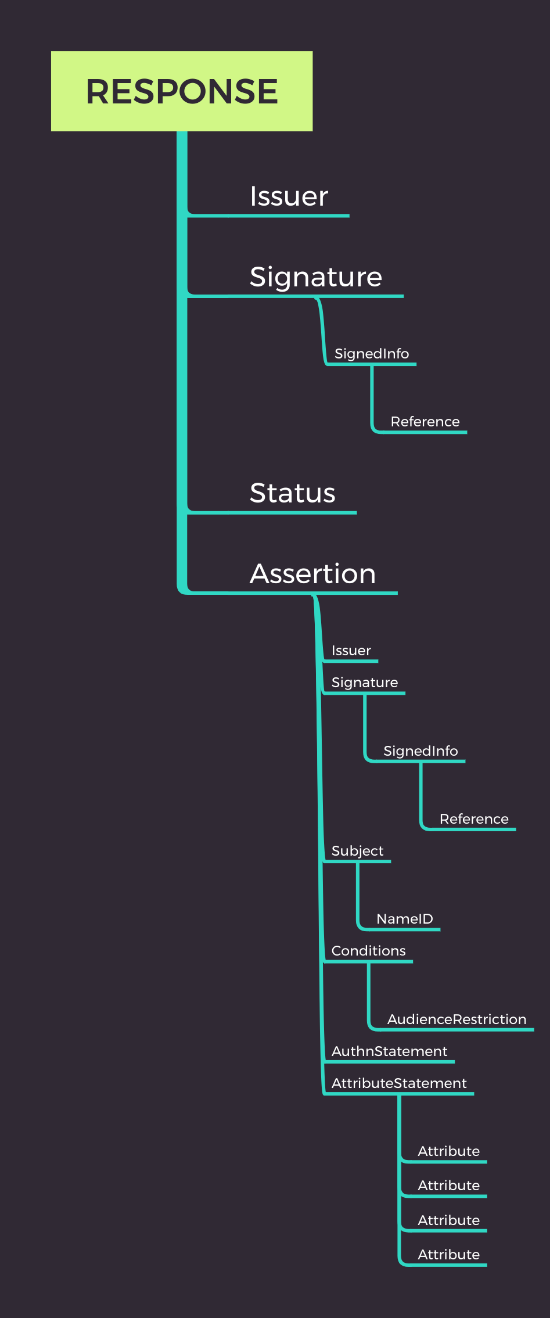
\includegraphics[width=\linewidth]{web_server_side/saml/images/response-layout.png}
  \caption{SAML response layout}
  \label{fig:saml-response-layout}
\end{figure}

Now that we’ve authenticated with the IdP and it has generated the SAML
Response above, it responds to our authentication with another 302 redirect

\begin{verbatim}
HTTP/1.1 302 Moved Temporarily
Date: Tue, 12 Mar 2019 20:54:53 GMT
Expires: 0
Cache-Control: no-cache, no-store, must-revalidate, max-age=0
Pragma: no-cache
Set-Cookie: _idp_session=MTkyLjE2OC4xLjk2%7CNmE1OWIwOTkxMjkzZjMyOTk2Yjg3NzE0NWNjYTkwYTliNGM1NDViZjRkZDhmY2M5OGQ2NmVjOGZlZTc0NzY1Ng%3D%3D%7CXWP3eN6ZeRPWk%2Bnj5AhRklHyIyU%3D; Version=1; Path=/idp; Secure
Location: https://shibdemo-idp.test.edu:443/idp/profile/SAML2/Redirect/SSO
Content-Length: 0
Connection: close
Content-Type: text/plain; charset=UTF-8
\end{verbatim}

The 302 ultimately leads to us making a POST request to the Service Provider’s
Assertion Consumer Service URL. The POST body contains the RelayState and
SAMLResponse parameters. Recall that the ACS processes and validates the SAML
Response.

\begin{verbatim}
POST /Shibboleth.sso/SAML2/POST HTTP/1.1
Host: shibdemo-sp1.test.edu
User-Agent: Mozilla/5.0 (X11; Ubuntu; Linux x86_64; rv:65.0) Gecko/20100101 Firefox/65.0
Accept: text/html,application/xhtml+xml,application/xml;q=0.9,image/webp,*/*;q=0.8
Accept-Language: en-US,en;q=0.5
Accept-Encoding: gzip, deflate
Referer: https://shibdemo-idp.test.edu/idp/profile/SAML2/Redirect/SSO
Content-Type: application/x-www-form-urlencoded
Content-Length: 12314
Connection: close
Upgrade-Insecure-Requests: 1

RelayState=ss%3Amem%3A39430bdac29d44586c326f12b4.. .SNIP. ..
\end{verbatim}

Once the POST request is received, and the SAML Response is validated, we can
access the protected resource we initially requested.

\begin{verbatim}
GET /secure/ HTTP/1.1
Host: shibdemo-sp1.test.edu
User-Agent: Mozilla/5.0 (X11; Ubuntu; Linux x86_64; rv:65.0) Gecko/20100101 Firefox/65.0
Accept: text/html,application/xhtml+xml,application/xml;q=0.9,image/webp,*/*;q=0.8
Accept-Language: en-US,en;q=0.5
Accept-Encoding: gzip, deflate
Referer: https://shibdemo-idp.test.edu/idp/profile/SAML2/Redirect/SSO
Connection: close
Cookie: _shibsession_64656661756c7468747470733a2f2f7368696264656d6f2d7370312e746573742e6564752f73686962626f6c657468=_ac05716a62d3ee9450c863b093f32bbb
Upgrade-Insecure-Requests: 1
\end{verbatim}

\begin{verbatim}
HTTP/1.1 200 OK
Date: Tue, 12 Mar 2019 20:55:04 GMT
Server: Apache/2.2.3 (CentOS)
X-Powered-By: PHP/5.1.6
Content-Length: 1047
Connection: close
Content-Type: text/html; charset=UTF-8


<?xml version="1.0" encoding="iso-8859-1"?>
<!DOCTYPE html PUBLIC "-//W3C//DTD XHTML 1.0 Transitional//EN" "http://www.w3.org/TR/xhtml1/DTD/xhtml1-transitional.dtd">
<html xmlns="http://www.w3.org/1999/xhtml">
<head>
<title>IDM Integration</title>
-------------8<-------------
\end{verbatim}

\subsection{XML Signatures}
Interestingly, XML Signatures can be used to sign either a whole XML tree or
specific elements within the tree. We already saw earlier that two separate XML
Signatures were used in our example SAML Response. Each signature was
responsible for a different part of the Response. In this section, we’ll look
at the different ways an XML Signature can be incorporated into an XML
document. Something to note is that while our examples use the Response element
as the resource to be signed, XML Signatures can be applied to any Object,
including Assertion elements.

\subsubsection{Enveloped signature}
A basic XML Signature is comprised of the following elements:
\begin{verbatim}
<Signature>
  <SignedInfo>
    <CanonicalizationMethod />
    <SignatureMethod />
    <Reference>
       <Transforms />
       <DigestMethod />
       <DigestValue />
    </Reference>
    <Reference />
  </SignedInfo>
  <SignatureValue />
  <KeyInfo />
  <Object />
</Signature>
\end{verbatim}
Of particular note for us is that each resource to be signed has its own
Reference element. The Reference element’s URI attribute denotes which resource
is signed by that particular Signature. By examining our example from earlier,
we can see this in practice.

\begin{verbatim}
<samlp:Response ... ID="_2af3ff4a06aa82058f0eaa8ae7866541" ... >
    ...
    <ds:Signature>
        <ds:SignedInfo>
            ...
            <ds:Reference URI="#_2af3ff4a06aa82058f0eaa8ae7866541">
                ...
            </ds:Reference>
        </ds:SignedInfo>
    </ds:Signature>
    ...
</samlp:Response>
\end{verbatim}
What we saw in our example earlier is known as an enveloped signature. An
enveloped signature is a signature that is a descendant of the resource it’s
signing. We can see that spelled out for us in the \verb+ds:Transform+ element
of our example.
\begin{verbatim}
<ds:Reference URI="#_2af3ff4a06aa82058f0eaa8ae7866541">
    <ds:Transforms>
        <ds:Transform Algorithm="http://www.w3.org/2000/09/xmldsig#enveloped-signature"/>
        ...
    </ds:Transforms>
    ...
</ds:Reference>
\end{verbatim}

\subsubsection{Enveloping signature}
In enveloping signatures the signature wraps the resource.

\begin{verbatim}
<ds:Signature>
    <ds:SignedInfo>
        ...
        <ds:Reference URI="#_2af3ff4a06aa82058f0eaa8ae7866541">
            ...
        </ds:Reference>
    </ds:SignedInfo>
    <samlp:Response ... ID="_2af3ff4a06aa82058f0eaa8ae7866541" ... >
        ...
    </samlp:Response>
</ds:Signature>
\end{verbatim}

\subsubsection{Detached signature}
Finally, there are detached signatures. A detached signature is neither
wrapping nor is it wrapped by the resource to be signed. Instead, it is wholly
separate from the signed resource.

\begin{verbatim}
<samlp:Response ... ID="_2af3ff4a06aa82058f0eaa8ae7866541" ... >
    ...
</samlp:Response>
<ds:Signature>
    <ds:SignedInfo>
        ...
        <ds:Reference URI="#_2af3ff4a06aa82058f0eaa8ae7866541">
            ...
        </ds:Reference>
    </ds:SignedInfo>
</ds:Signature>
\end{verbatim}

\subsection{Attack methodology}
\begin{figure}
  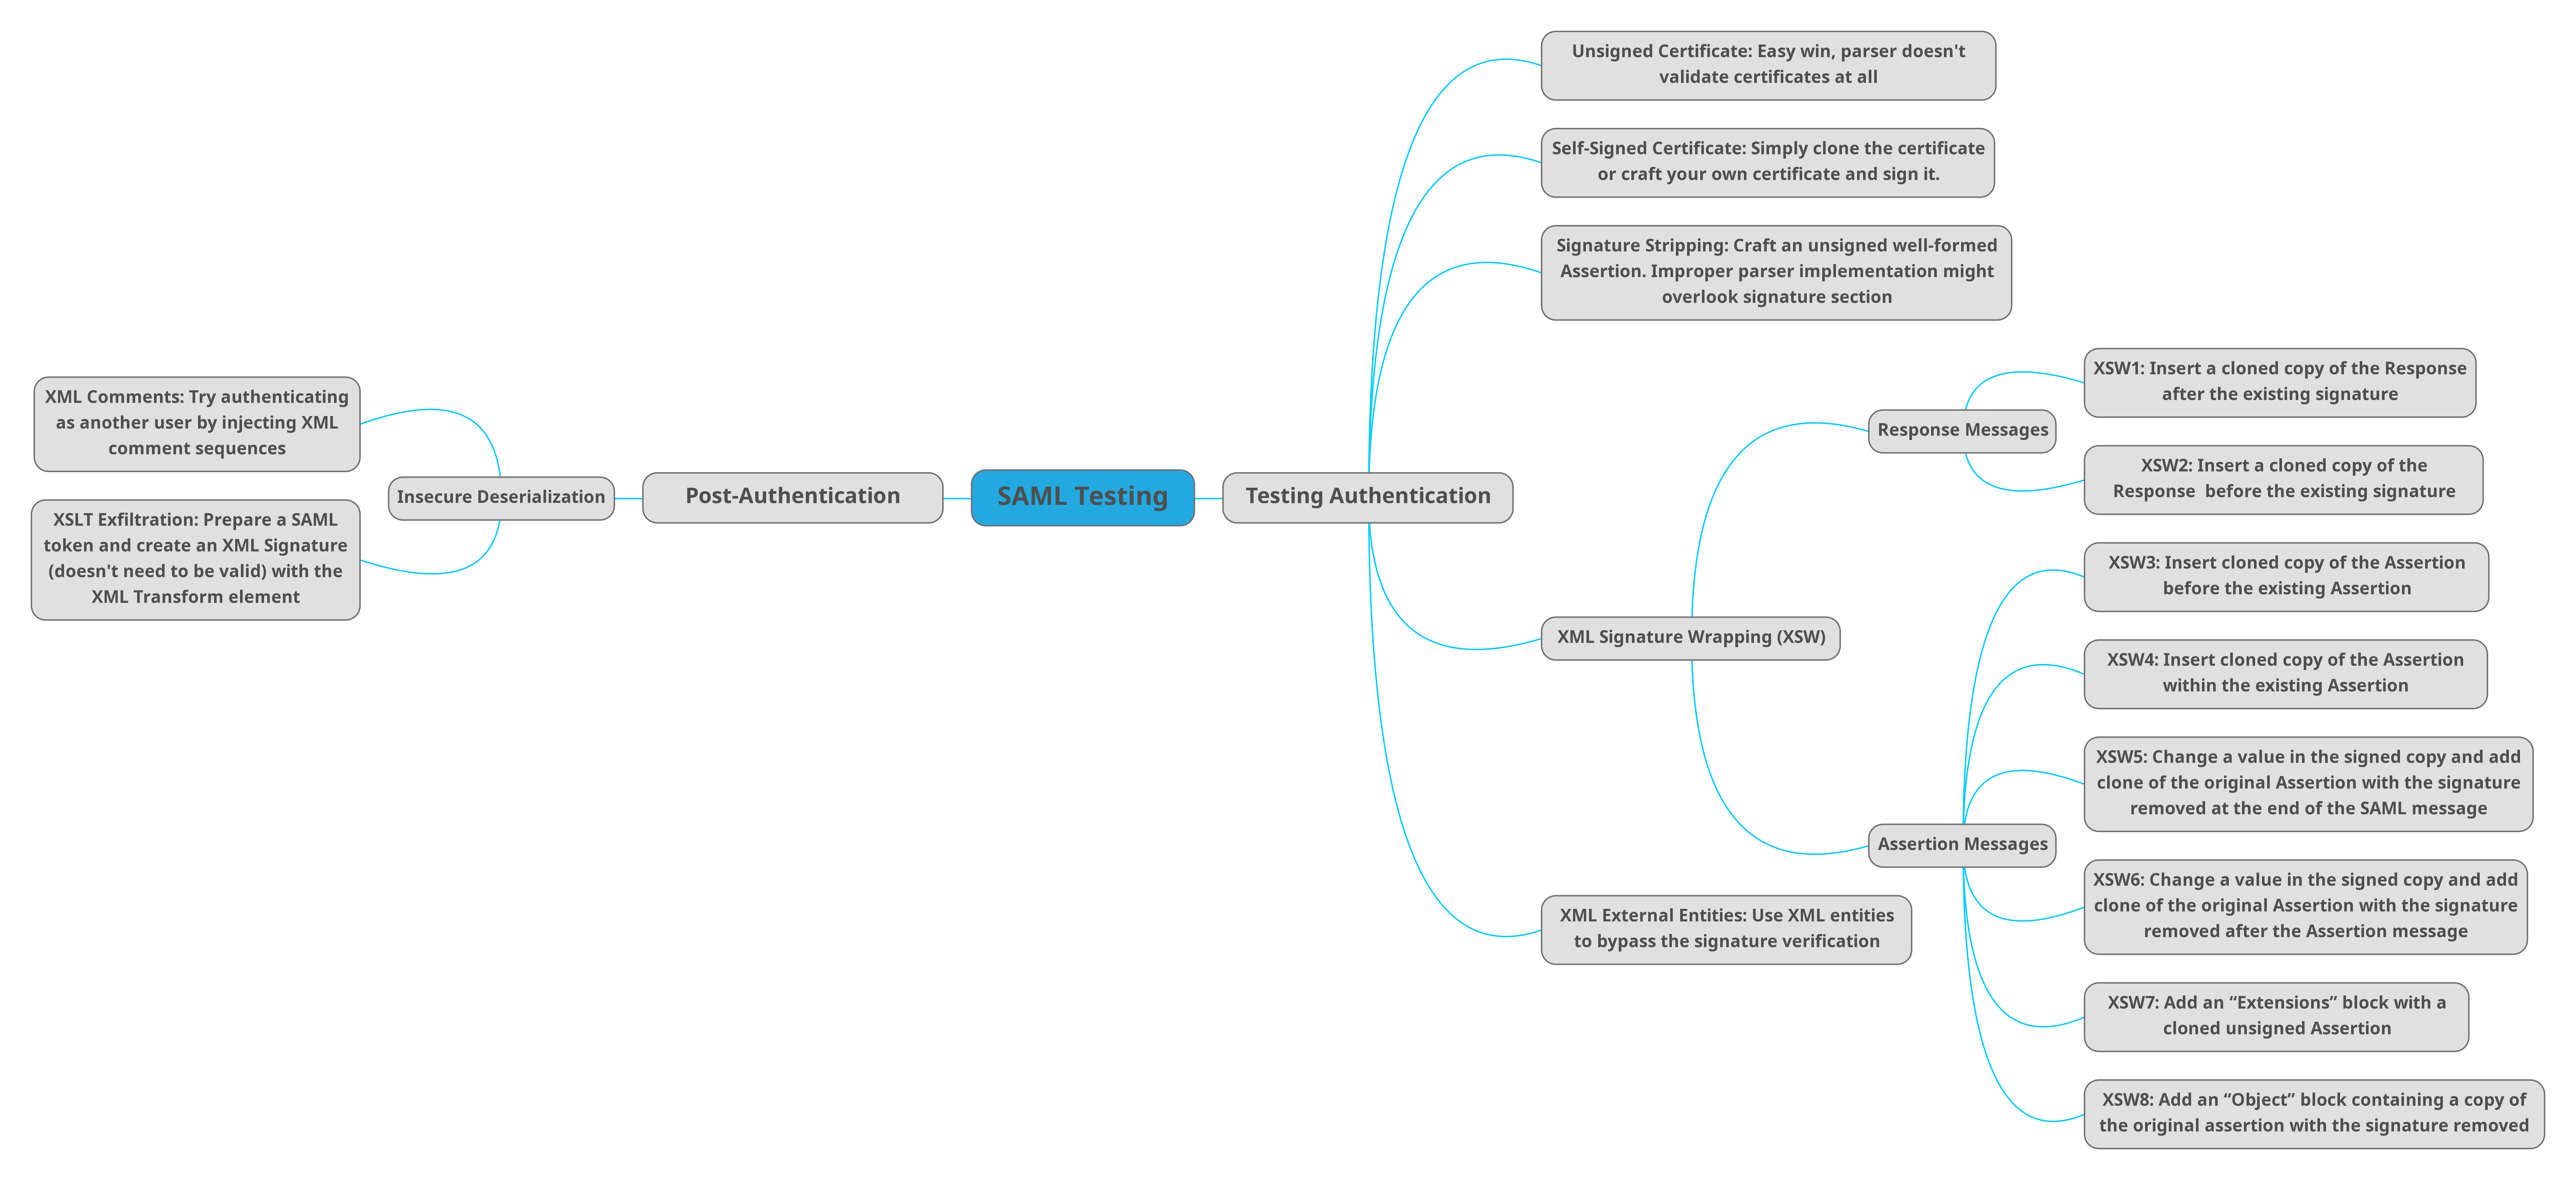
\includegraphics[width=\linewidth]{web_server_side/saml/images/attacks.png}
  \caption{SAML v2 attacks}
  \label{fig:saml-attacks}
\end{figure}
